\begin{figure}
\centering
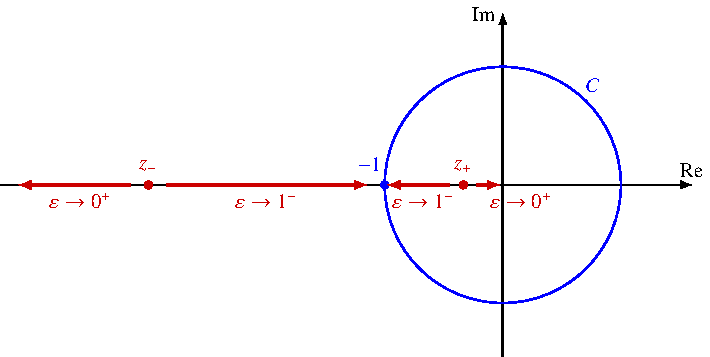
\includegraphics{papers/kepler/images/polstellen.pdf}
\caption{Lage der beiden Polstellen relativ zum Integrationsweg $C$.
Gezeichnet ist der Fall $\varepsilon=0.6$.
Beide Polstellen liegen auf der negativen reellen Achse, hier bei $z_+=-\frac13$ und $z_-=-3$.
Nur $z_+$ liegt im Inneren des Einheitskreises.
Nur dieser Pol trägt zum Wegintegral bei.
Die roten Pfeile deuten das Verhalten bei Veränderung von $\varepsilon$ an.
Für $\varepsilon\to 1^-$ streben beide Pole gegen den Punkt $-1$ auf dem Einheitskreis.
\label{kepler:figure:polstellen}}
\end{figure}
